\section{Oscilador de Wien}
\subsection{Introducción}
Las señales senoidales son de vital importancia en el ámbito de la electrónica, tanto en usos de intercambio de información como transferencia de energía, entre otros, y 
es justamente por eso que la generación de las mismas es de real importancia.
Una forma de generar señales senoidales mediante componentes analógicos electrónicos es mediante osciladores, y uno de los ejemplos de estos circuitos es el oscilador de 
Wien, cuya forma más elemental se muestra en la Figura \ref{fig:basic_wien_osc}.
\begin{figure}[H]
    \centering
    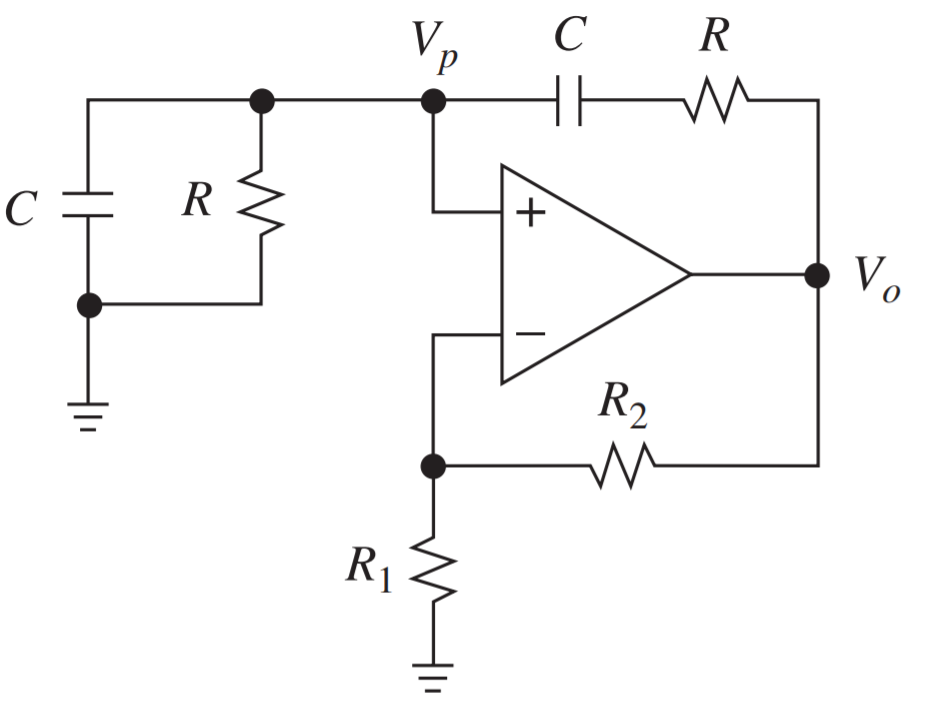
\includegraphics[width=0.5\textwidth]{../EJ1/Recursos/basic_wien_osc.png}
    \caption{Oscilador de Wien en su forma más sencilla.}
    \label{fig:basic_wien_osc_ex1}
\end{figure}
El objetivo de esta sección del artículo es, basándose en derivaciones del circuito anterior, diseñar un oscilador que genere una señal senoidal con su frecuencia de 
oscilación en $77.5KHz$ como único parámetro de diseño.



\subsection{Marco teórico}
\subsubsection{Frecuencia de oscilación}
Retomando el circuito planteado en la sección anterior, el mismo puede ser analizado para encontrar las relaciones que determinan el los parámetros fundamentales de la 
señal generada por el oscilador.
El mismo puede ser pensado como un amplificador realimentado tanto positiva como negativamente, donde el lazo negativo es el de un amplificador no inversor de ganancia:
\begin{align} 
    & A = 1 + \frac{R_2}{R_1}
    \label{eq:neg_loop_gain_ex1}
\end{align}

La tensión de entrada a este no inversor puede ser puesta en función de los parámetros del lazo negativo mediante la ecuación \ref{eq:v_p_by_v_o_ex1}.
\begin{align*}
    & V_p = V_o \frac{R // \frac{1}{j \cdot 2\pi \cdot f \cdot C}}{\left( R // \frac{1}{j \cdot 2\pi \cdot f \cdot C} \right) + \left( R + \frac{1}{j \cdot 2\pi \cdot f \cdot C}\right)}
\end{align*}
Manipulando algebraicamente esta expresión se obtiene la ganancia debida al lazo positivo:
\begin{align}
    & B(jf) = \frac{1}{3 + j \cdot \left(\frac{f}{f_0} - \frac{f_0}{f}\right)}
    \label{eq:pos_loop_gain_ex1}
\end{align}
Donde:
\begin{align}
    & f_0 = \frac{1}{j \cdot 2\pi \cdot R \cdot C}
    \label{eq:osc_freq_ex1}
\end{align}

La ganancia total del oscilador viene dada por la multiplicación de las ganancias de los lazos, consecuentemente, de las ecuaciones \ref{eq:neg_loop_gain_ex1} y \ref{eq:pos_loop_gain_ex1}
se obtiene:
\begin{align}
    & T(jf) = \frac{1 + \frac{R_2}{R_1}}{3 + j \cdot \left(\frac{f}{f_0} - \frac{f_0}{f}\right)}
    \label{eq:total_gain_ex1}
\end{align}

De la observación de esta transferencia puede deducirse que se trata de un pasa banda con ganancia máxima en $f = f_0$ y ganancia:
\begin{align}
    & T_{max} = \frac{1 + \frac{R_2}{R_1}}{3}
    \label{eq:max_gain_ex1}
\end{align}


\subsubsection{Criterio de Barkhausen}
El criterio de Barkhausen dicta las condiciones que deben cumplirse en oscilador como el de Wien para que se cumpla la condición de oscilación y determina la frecuencia a 
la que se dará el mismo.
El criterio consiste en hallar el punto para el cual se cumple que la ganancia es 1 y el desfasaje es nulo, y, para el circuito en cuestión, observamos que la segunda de 
las condiciones puede ser cumplida evaluando en $f_0$, mientras que la primera puede cumplirse para esa misma frecuencia si $\frac{R_2}{R_1} = 2$


\subsubsection{Desviaciones del circuito básico}
Si bien el circuito previamente mencionado puede ser utilizado para buscar de forma más sencilla las relaciones que determinan el cumplimiento o no de la oscilación, en 
la práctica deben de hacerse modificaciones que prevengan al circuito de las variaciones intrínsecas a la utilización de componentes reales.
Como se dijo en la sección anterior, para que se cumpla el criterio de Barkausen, debe darse que $\frac{R_2}{R_1} = 2$ exactamente; sin embargo, esta característica no 
puede ser lograda en la realidad con simples componentes pasivos, razón por la cual el circuito original de la Figura \ref{fig:basic_wien_osc_ex1}, es reemplazado por el 
de la Figura \ref{fig:wein_osc_circuit_ex1}.
\begin{figure}[H]
    \centering
    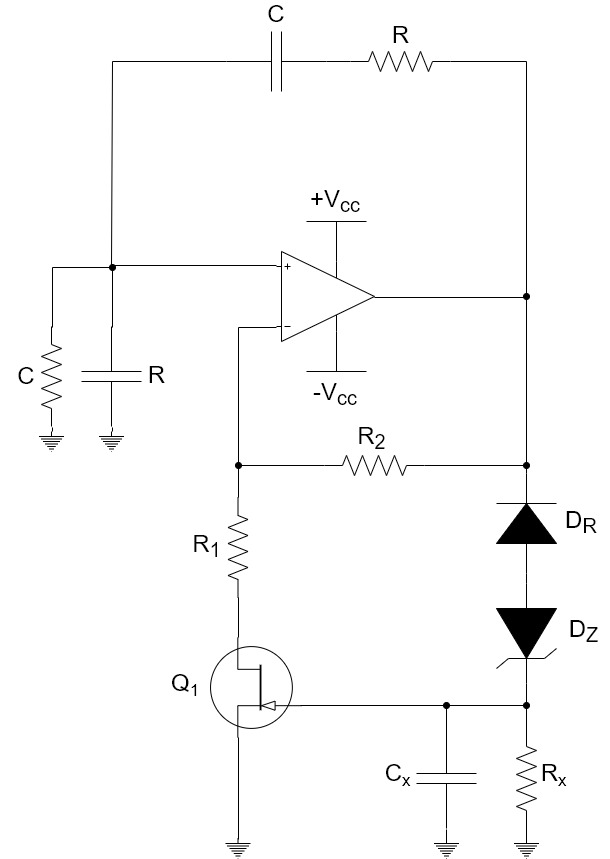
\includegraphics[width=0.5\textwidth]{../EJ1/Recursos/wein_osc_circuit.jpg}
    \caption{Circuito utilizado.}
    \label{fig:wein_osc_circuit_ex1}
\end{figure}

\textbf{Transistor JFET}\\
La principal diferencia yace en la inclusión de un JFET-N en la realimentación negativa, en serie con $R_1$, cuya función es la de resistencia variable 
dinámicamente.
Mediante esta incorporación, puede colocarse una resistencia en $R_1$ de valor tal que $\frac{R_2}{R_1} > 2$ que en el encendido del circuito favorezca 
la realimentación positiva, y se inicie la oscilación.
Una vez llegado al valor deseado de tensión de salida de la señal (fijado por los diodos, y explicado en el siguiente ítem), la tensión en el Gate del 
transistor se modificará achicando el ancho del canal y aumentando entonces la resistencia del mismo.
Con este mecanismo es que se logra que la ganancia del lazo negativo llegue a la condición de $\frac{R_2}{R_1} = 2$.

La elección de qué tipo de JFET se usa va de la mano de la disposición de los diodos.
Cabe recordar que un JFET canal N disminuirá el ancho de su canal conforme se aplique tensión negativa en su Gate, mientras que el canal P lo hará ante 
tensiones de valor positivo.
Consecuentemente, el uso de un canal N realizará un control de la oscilación a través del semiciclo negativo de la misma, mientras que un canal P lo hará 
para el positivo.

Otro aspecto a considerar es la zona de utilización del transistor y el rango de variación de la tensión en el Gate.
Este JFET está siendo usado en la zona lineal, con bajas tensiones en el Gate, empleándose como resistencia variable.
En cuanto a la variación de estas tensiones, se pretende que sean chicas, ya que la no linealidad en la respuesta del transistor podría introducir 
distorsiones en caso de que no lo fueran.

\textbf{Diodo rectificador y Zener ($D_R$ y $D_Z$)}
Su función, como bien se mencionó antes, es la de limitar la amplitud de la señal generada a la salida.
Cada vez que la salida del operacional supera el valor dado por $V_Z + V_D$, más la tensión en el capacitor cargado, los diodos limitan la amplitud a la 
salida.
En el circuito de la Figura \ref{fig:wein_osc_circuit_ex1}, los diodos están dispuestos de forma tal que la limitación de la amplitud se dé en el 
semiciclo negativo, dado que se está utilizando un JFET canal N para el control de la ganancia del lazo negativo.
En caso de querer usar un JFET canal P, ambos deberían ser invertidos en su conexión, para permitir el control en el semiciclo positivo.

\textbf{Capacitor y resistencia $R_x$ y $C_x$}
Esta malla RC, la cual puede ser vista como un pasa-bajos, cumple la función de mantener la polarización del transistor JFET durante todo el ciclo de la 
senoidal.
Se busca que la constante de tiempo del mismo sea alta, para lograr así el deseado efecto de que la variación en la tensión de Gate sea baja, y esto se 
logra colocando valores altos de $R_x$.



\subsection{Diseño y función de los componentes}
\subsubsection{Lazo de realimentación positiva}



\subsubsection{Lazo de realimentación negativa}


\subsubsection{Diodo rectificador y diodo Zener}


\subsubsection{Transistor JFET}


\subsubsection{Polarización del JFET ($C_3$ y $R_x$)}


\subsubsection{Selección del operacional a utilizar}



\subsection{Caracterización del sistema}
\subsubsection{Singularidades}


\subsubsection{Sensibilidades}



\subsection{Resultados}
\subsubsection{Frecuencia de oscilación}


\subsubsection{Tensión de salida}


\subsubsection{Establecimiento de la señal}


\subsubsection{Distorsión armónica}
